		
\subsection*{Введение}

Цель работы заключается в изучении температурной зависимости магнитной восприимчивости ферромагнетика выше точки Кюри.

Для этого используются катушка самоиндукции с образцом из гадолиния, термостат, частотомер, цифровой вольтметр, LC-автогенератор, термопара медь-константан.

\subsection*{Теоретическая справка}

При стремлении температуры к нулю тепловое движение все меньше препятствует магнитным моментам атомов ориентироваться в соответствии со внешнем магнитным полем. В ферромагнетиках это происходит при понижении температуры не до нуля, а до температуры Кюри $\theta$. Для ферромагнетиков закон Кюри (1) должен быть заменен на закон Кюри-Вейсса (2), где $\theta_p$ -- некоторая близкая к $\theta$ температура, называемая парамагнитной точкой Кюри. 

\begin{equation}
	\chi = \frac{C}{T},
\end{equation}

\begin{equation}
	\chi \sim \frac{1}{T - \theta_p},
\end{equation}

\subsubsection*{Экспериментальная установка}

\begin{figure}[hbt]\label{risI}
    \center{\includegraphics[scale=1]{lab342ris1.png}}
    \caption{\textit{Схема экспериментальной установки}}
\end{figure}

Исследуемый ферромагнитный образец -- в нашем случае гадолиний -- располагается внутри пустотелой катушки самоиндукции входящей в состав LC-автогенератора, который собран на полевом транзисторе КП-103 и выделен в отдельный блок. 

Ввиду хорошей проводимости гадолиния и высокой рабочей частоты генератора ($\sim$ 50кГц) образец изготавливается из мелких кусочков размером около 0,5мм -- для уменьшения вихревых потоков. Катушка 1 с образцом помещена в стеклянный сосуд 2, залитый трансформаторным маслом, которое призвано улучшить тепловой контакт между образцом и термостатируемой жидкостью 3. В емкость вмонитрован термометр 4.

Обозначив за $L$ самоиндукцию катушки с образцом и через $L_0$ -- самоиндукцию в отсутствиие образца, получим:

\begin{equation}
    (L-L_0) \sim \chi.    
\end{equation}

По формуле Томсона период колебаний автогенератора с емкостью контура автогенератора C:

\begin{equation}
    \tau = 2 \pi \sqrt{LC}, \,\
    \tau = 2 \pi \sqrt{L_0C}.
\end{equation}

Тогда из (4) получаем:

\begin{equation}
    (L - L_0) \sim (\tau^2 - \tau_0^2) \longrightarrow \chi \sim (\tau^2 - \tau_0^2).
\end{equation}

Тогда получаем, что закон Кюри-Вейсса справедлив, если выполнено соотношение:

\begin{equation}
    \frac{1}{\chi} \sim (T - \theta_p) \sim \frac{1}{(\tau^2 - \tau_0^2)}.
\end{equation}

Величина стабилизирующей температуры задаётся на дисплее 5 термостата. Для нагрева служит внутренний электронагреватель, для охлаждения циркуллирующая водопроводная вода. 

\subsection*{Ход работы}

Подготовим приборы к работе. Оценим допустимую ЭДС термопары, если допустимая разность температур образца и рабочей жидкости $\Delta T = 0,5 ^\circ C$, а постоянная термопары $k = 24 \, град/мВ$ :

\begin{equation}
    U_m = \frac{\Delta T}{k} \approx 0,021мВ.
\end{equation}

Исследуем зависимость периода колебаний LC - генератора от температуры образца, отмечая период колебаний $\tau$ по частотомеру, а температуру T -- по показаниям дисплея и цифровому вольтметру. Проведем измерения в диапазоне от $14 ^\circ C$ до $40 ^\circ C$ через $2 ^\circ C$. Результаты отразим в таблице 1.

\subsection*{Обработка результатов}

В столбце "$T, ^\circ C$" указаны температуры, снятые с дисплея термостата -- их погрешность оценивается в $0,05 ^\circ C$. В столбце "$\varepsilon, мВ$" указаны показания вольтметра, снимающего разность ЭДС на термопаре. В столбце "$\tau, мкс$" указаны периоды колебаний LC-контура при данной температуре. Столбец "$T_{real}, ^\circ C$" истинные значения температур -- она складывается из температуры термостата и разности ЭДС на термопаре. Как видно, разница между $T$ и $T_{real}$ действительно не превышает указаний из формулы (7).

Для изучения зависимости (6) рассчитаем точки по данным из таблицы 1 и результаты вместе с погрешностями укажем в таблице 2. 

Из графика видно, что, только первые две точки можно считать лежащими на одной горизонтальной прямой. Далее идёт нелинейный рост, которым, видимо, как промежуточным процессом, теория пренебрегает. После $20 ^\circ C$ становится очевидным линейность зависимости. Из графика определяем уравнение аппроксимирующей прямой, вычисляем искомую температуру:

\begin{equation}
    \theta_p = (17,83\pm0,83) ^\circ C.
\end{equation}

\subsection*{Обсуждение результатов}

Итоговое значение температуры точки Кюри для гадолиния вышло ниже табличного значения на $\approx 1 ^\circ C$. Как видно из графика, занижению результата способствуют последние две точки, выпадающие из линейной аппроксимации.


\begin{table}[hbt]
\centering
\begin{tabular}{|c|c|c|c|}
\hline
\textbf{$T,   ^\circ C$} & \textbf{$\varepsilon, мВ$} & \textbf{$\tau, мкс$} & \textbf{$T_{real}, ^\circ C$} \\ \hline
12,190                   & -0,005                     & 7,970                & 12,068                        \\ \hline
14,140                   & -0,008                     & 7,935                & 13,943                        \\ \hline
16,110                   & -0,019                     & 7,885                & 15,644                        \\ \hline
17,060                   & -0,021                     & 7,846                & 16,561                        \\ \hline
18,110                   & -0,010                     & 7,766                & 17,880                        \\ \hline
19,050                   & -0,021                     & 7,718                & 18,548                        \\ \hline
20,070                   & -0,021                     & 7,627                & 19,561                        \\ \hline
22,080                   & -0,020                     & 7,439                & 21,607                        \\ \hline
24,080                   & -0,021                     & 7,239                & 23,581                        \\ \hline
26,080                   & -0,019                     & 7,152                & 25,624                        \\ \hline
28,070                   & -0,019                     & 7,109                & 27,621                        \\ \hline
30,050                   & -0,021                     & 7,083                & 29,556                        \\ \hline
32,060                   & -0,021                     & 7,063                & 31,568                        \\ \hline
34,070                   & -0,019                     & 7,048                & 33,619                        \\ \hline
36,060                   & -0,021                     & 7,038                & 35,561                        \\ \hline
\end{tabular}
\caption{Результаты измерений}
\end{table}
\begin{table}[hbt]
    \centering
\begin{tabular}{|c|c|c|c|}
\hline
\textbf{$T_{real},   ^\circ C$} & \textbf{$\sigma_{\tau}, мкс$} & \textbf{$\frac{1}{(\tau^2-\tau_0^2)}=f(\tau),   мкс^{-2}$} & \textbf{$\sigma_{\frac{1}{\tau^2-\tau_0^2}},   мкс^{-2}$} \\ \hline
12,07                           & 0,01                          & 0,063                                                      & 0,001                                                      \\ \hline
13,94                           & 0,01                          & 0,066                                                      & 0,001                                                      \\ \hline
15,64                           & 0,01                          & 0,069                                                      & 0,001                                                      \\ \hline
16,56                           & 0,01                          & 0,072                                                      & 0,001                                                      \\ \hline
17,88                           & 0,01                          & 0,080                                                      & 0,001                                                      \\ \hline
18,55                           & 0,01                          & 0,085                                                      & 0,001                                                      \\ \hline
19,56                           & 0,01                          & 0,096                                                      & 0,001                                                      \\ \hline
21,61                           & 0,01                          & 0,132                                                      & 0,003                                                      \\ \hline
23,58                           & 0,01                          & 0,214                                                      & 0,007                                                      \\ \hline
25,62                           & 0,01                          & 0,293                                                      & 0,012                                                      \\ \hline
27,62                           & 0,01                          & 0,357                                                      & 0,018                                                      \\ \hline
29,56                           & 0,01                          & 0,412                                                      & 0,024                                                      \\ \hline
31,57                           & 0,01                          & 0,466                                                      & 0,031                                                      \\ \hline
33,62                           & 0,01                          & 0,515                                                      & 0,037                                                      \\ \hline
35,56                           & 0,01                          & 0,556                                                      & 0,043                                                      \\ \hline
\end{tabular}
\caption{Данные для графика}
\end{table}

\begin{figure}[hbt]
    \centering
    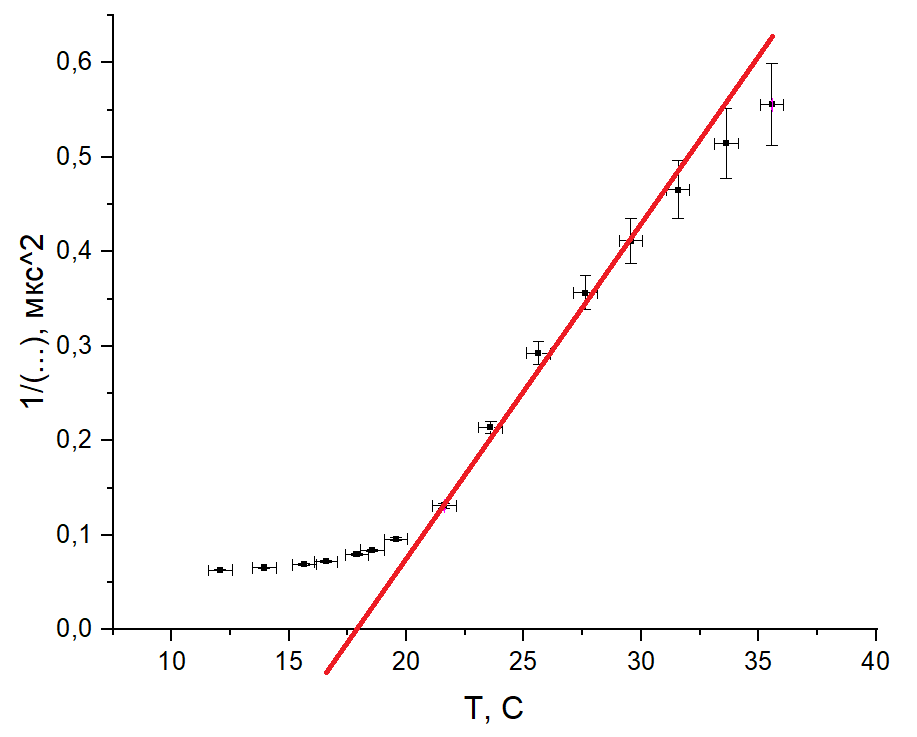
\includegraphics[scale = 0.8]{lab324ris2.png}
    \caption{Данные таблицы 1. По вертикальной оси $\frac{1}{\tau^2-\tau_0^2}, мкс^{-2}$, по горизонтальной $T_{real}, ^\circ C$. Уравнение аппроксимированной прямой -- $f(T) = (0,035\pm0,002)\cdot T_{real} + (-0,631\pm0,036), мкс^{-2}$}
\end{figure}


\end{document}

